\documentclass[12pt]{article}
\usepackage{graphicx} % Required for inserting images
\usepackage[margin=2cm, symmetric]{geometry}
\usepackage{listings}
\usepackage{xcolor}
\usepackage{color}
\usepackage{tabularx}
\usepackage{booktabs} 
\usepackage{graphicx}
\usepackage{amsmath}
\usepackage{afterpage}
\usepackage{float}
\usepackage{placeins}
\usepackage{fancyvrb}


\linespread{1.5}

\definecolor{light-gray}{gray}{0.65}
\definecolor{codegreen}{rgb}{0,0.6,0}
\definecolor{codegray}{rgb}{0.5,0.5,0.5}
\definecolor{codepurple}{rgb}{0.58,0,0.82}
\definecolor{backcolour}{rgb}{0.95,0.95,0.92}

\lstdefinestyle{mystyle}{
    language=R, % Specify the language for syntax highlighting
    backgroundcolor=\color{backcolour},   
    commentstyle=\color{codegreen},
    keywordstyle=\color{magenta},
    numberstyle=\tiny\color{codegray},
    stringstyle=\color{codepurple},
    basicstyle=\footnotesize,
    breakatwhitespace=false,         
    breaklines=true,                 
    captionpos=b,                    
    keepspaces=true,                 
    numbers=left,                    
    numbersep=5pt,                  
    showspaces=false,                
    showstringspaces=false,
    showtabs=false,                  
    tabsize=2
}
\lstset{style=mystyle}

\newcommand{\Sref}[1]{Section~\ref{#1}}
\newtheorem{hyp}{Hypothesis}

\title{Problem Set 3}
\author{Yajie Dong}
\date{19th November 2023}

\begin{document}

\maketitle

\section{Question 1}
\subsection{Run a regression where the outcome variable is voteshare and the explanatory variable is difflog.}

\textbf{Step 1: Import the dataset using the read.csv() function.}

Do it in R:
\begin{lstlisting}
inc.sub <- read.csv("https://raw.githubusercontent.com/ASDS-TCD/StatsI_Fall2023/main/datasets/incumbents_subset.csv")
\end{lstlisting}

\textbf{Step 2: Rename 'voteshare' to 'Y' and 'difflog' to 'X1'. }

Do it in R:
\begin{lstlisting}
# Rename the 'voteshare' column to 'Y' and 'difflog' to 'X1' for easier reference.
names(inc.sub)[names(inc.sub) == "voteshare"] <- "Y"
names(inc.sub)[names(inc.sub) == "difflog"] <- "X1"
\end{lstlisting}


\textbf{Step 3: Run the Linear Regression:Fit a linear model with 'Y' as the dependent variable and 'X1' as the independent variable using the lm() function.}

Do it in R:

\lstset{style=mystyle}
\begin{lstlisting}
model <- lm(Y ~ X1, data=inc.sub)
\end{lstlisting}
This may represent the linear relationship:
\begin{equation}
    Y = \alpha + \beta X_1 + \epsilon,
\end{equation}
where \( \alpha \) is the intercept, \( \beta \) is the slope, and \( \epsilon \) is the error term.

\textbf{Step 4:Output a summary of the linear regression model to get detailed statistics.} Do it in R:
 \lstset{style=mystyle}
\begin{lstlisting}
 summary(model)
\end{lstlisting}

\textbf{Generate and display a summary of the linear regression model using R:}
\begin{center}
\begin{BVerbatim}
    Call:
lm(formula = Y ~ X1, data = inc.sub)

Residuals:
     Min       1Q   Median       3Q      Max 
-0.26832 -0.05345 -0.00377  0.04780  0.32749 

Coefficients:
            Estimate Std. Error t value Pr(>|t|)    
(Intercept) 0.579031   0.002251  257.19   <2e-16 ***
X1          0.041666   0.000968   43.04   <2e-16 ***
---
Signif. codes:  0 ‘***’ 0.001 ‘**’ 0.01 ‘*’ 0.05 ‘.’ 0.1 ‘ ’ 1

Residual standard error: 0.07867 on 3191 degrees of freedom
Multiple R-squared:  0.3673,	Adjusted R-squared:  0.3671 
F-statistic:  1853 on 1 and 3191 DF,  p-value: < 2.2e-16

\end{BVerbatim}
\end{center}


\textbf{Use the R output to provide an explanation:}

 The \textbf{regression model }is defined by the formula \( \text{voteshare} \sim \text{difflog} \), indicating that \text{voteshare} is the dependent variable and \text{difflog} is the independent variable.


\textbf{Coefficients Interpretation:}
The coefficients are key components of our regression equation. The estimated intercept (\( \alpha \)) is 0.579031, and the estimated slope (\( \beta \)) for difflog (which we will call \( X1 \)) is 0.041666. Both coefficients are statistically significant with p-values less than 0.05.

\textbf{Model Fit:}
The residual standard error is 0.07867, indicating the standard deviation of the residuals. The R-squared value is 0.3673, meaning that approximately 36.73\% of the variance in voteshare is explained by difflog.

\textbf{F-Statistic:}
The F-statistic is 1853 with a p-value less than 2.2e-16, which is practically zero, indicating that the model is statistically significant.


 
\subsection{Make a scatterplot of the two variables and add the regression line.}
 Let's do it in R:
\lstset{style=mystyle}
\begin{lstlisting}
 # Create a scatterplot of 'X1' versus 'Y' using ggplot2 and add a linear regression line.
scatterplot <- ggplot(inc.sub, aes(x=X1, y=Y)) +
  geom_point(color = "#3498db", shape = 19, size = 2) + # A bright but soft blue color for points
  geom_smooth(method = "lm", color = "#e74c3c", se = FALSE, linetype = "solid", size = 1) + # A soft red for the regression line
  labs(title = "Vote Share vs. Campaign Spending Difference",
       x = "Logarithm of Campaign Spending Difference (X1)",
       y = "Incumbent's Vote Share (Y)") +
  theme_light() + # Use a light theme for a brighter background
  theme(
    plot.title = element_text(hjust = 0.5, size = 20, face = "bold"), # Center and bold the plot title
    axis.title.x = element_text(size = 14, face = "bold"), # Bold X axis title
    axis.title.y = element_text(size = 14, face = "bold"), # Bold Y axis title
    axis.text = element_text(size = 12, color = "#2c3e50"), # Dark text for better contrast
    axis.line = element_line(color = "#2c3e50"), # Dark axis lines for contrast
    panel.grid.major = element_line(color = "#bdc3c7", linetype = "dotted"), # Light gray for major grid lines
    panel.grid.minor = element_blank(), # Remove minor grid lines
    legend.position = "none" # Remove legend
  )

# Save the updated scatterplot as a PNG file
ggsave("scatterplot_Y_X1_regression_line.png", plot = scatterplot, width = 10, height = 8, dpi = 300)
\end{lstlisting}
\textbf{Now we have the scatterplot of the two variables and add the regression line:}
\begin{figure}[h!]
    \centering
    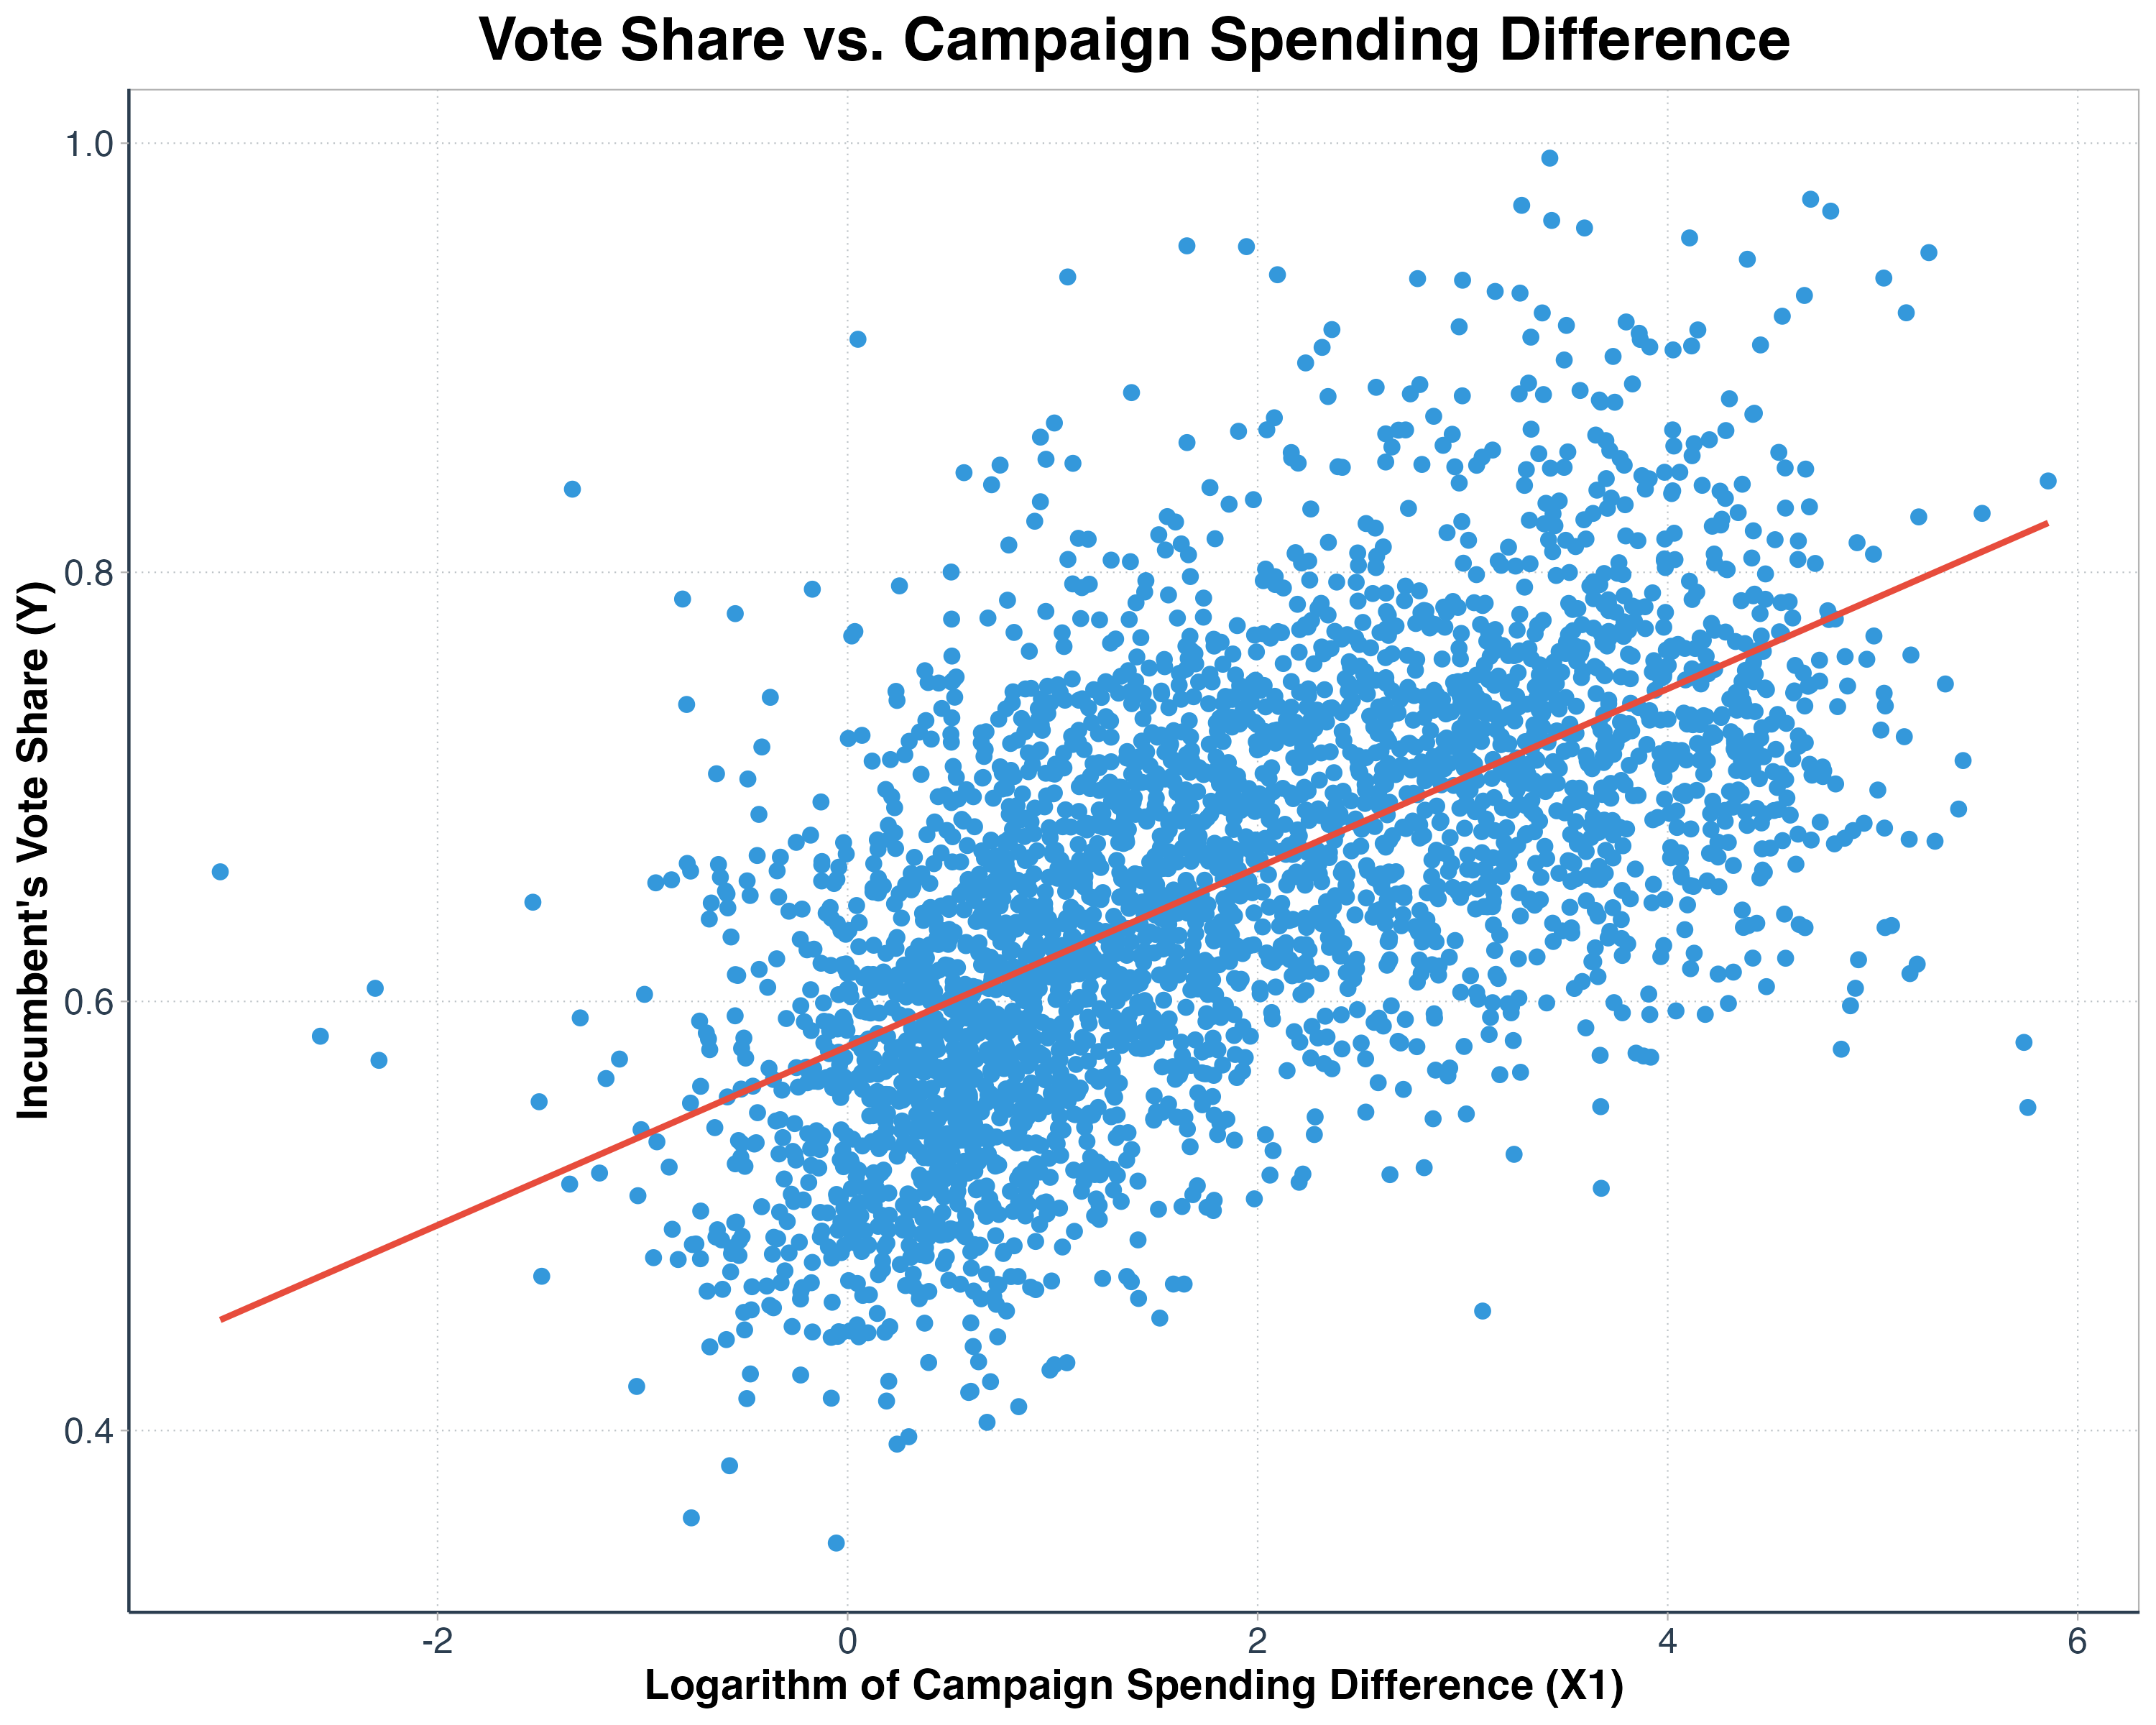
\includegraphics[width=.75\textwidth]{scatterplot_Y_X1_regression_line.png}
    \caption{\footnotesize Y and X1.}
    \label{fig:plot_1}
    \smallskip
    \raggedright
    \textbf{Scatterplot Interpretation:}
    
    The scatter plot above illustrates the relationship between the logarithm of campaign spending difference (X1) and the incumbent's vote share (Y). A moderate, positive linear correlation is observed between the two variables. The red line indicates the regression line, suggesting that as X1 increases, so generally does Y. However, the variability in the spread of data points along this line points to differences in the relationship's strength across the dataset, hinting at the influence of other factors.
\end{figure}

\newpage
\subsection{ Save the residuals of the model in a separate object.}
Do it in R:
\begin{lstlisting}
# Extract the residuals from the fitted model and store them in an object called 'residuals'.
# Residuals are the differences between observed values and values predicted by the model.
residuals <- resid(model)
# View the first few residuals using the head function to get an immediate sense of their distribution.
head(residuals)
# Get a summary of the residuals to understand their central tendency and spread.
summary(residuals)
\end{lstlisting}
\textbf{To represent R output in tabular form using LaTeX:}
\begin{table}[h!]
\centering
\begin{minipage}{.5\textwidth}
\centering
\begin{tabular}{|c|r|}
\hline
Observation & Residual \\
\hline
1 & -0.0004227622 \\
2 & -0.0316840149 \\
3 & -0.0045514943 \\
4 & 0.0386688767 \\
5 & 0.0355287965 \\
6 & 0.0322832521 \\
\hline
\end{tabular}
\caption{First six residuals of residuals\_Y\_X1.}
\label{tab:residuals}
\end{minipage}%
\begin{minipage}{.5\textwidth}
\centering
\begin{tabular}{|l|r|}
\hline
Statistic & Value \\
\hline
Minimum & -0.268319 \\
1st Quartile & -0.053454 \\
Median & -0.003769 \\
Mean & 0.000000 \\
3rd Quartile & 0.047798 \\
Maximum & 0.327488 \\
\hline
\end{tabular}
\caption{Summary statistics of residuals\_Y\_X1.}
\label{tab:summary_stats}
\end{minipage}
\end{table}

\textbf{Residuals Analysis:}

The head of the residuals shows individual differences between observed and predicted values for the first six observations. The summary of the residuals shows that their mean is 0, which is typical for linear regression.The mean of residuals being close to 0 in linear regression is a sign that the model is making predictions that are, on average, very close to the actual data points. This is an expected outcome when the linear regression model is a good fit for the data.

\subsection{ Write the prediction equation.}

From the model summary, we can extract the intercept and slope coefficients to create the prediction equation. Additionally, we have the option to utilize R for this purpose.

Let's do it in R:
\begin{lstlisting}
# Retrieve the intercept and slope coefficients from the model and store them in variables.
intercept <- coef(model)[1]
slope <- coef(model)[2]
# This equation can be used to predict 'Y' given new values of 'X1'.
prediction_equation_Y_X1 <- paste("Y =", format(intercept, digits = 4), "+", format(slope, digits = 4), "* X1")
print(prediction_equation_Y_X1)   
\end{lstlisting}

\textbf{Now we have the prediction equation:}
\begin{equation}
Y = 0.579 + 0.04167 \times X1
\end{equation}


\textbf{The explanation of the prediction equation:}

This equation suggests that the incumbent's vote share (\(Y\)) is positively influenced by the logged difference in campaign spending (\(X1\)). The incumbent's vote share is predicted to increase by 0.04167 for each one-unit increase in \(X1\).


\section{Question 2}
\subsection{Run a regression where the outcome variable is presvote and the explanatory variable is difflog.}

 \textbf{Step 1: Rename 'presvote' to 'X2' and 'difflog' to 'X1'.} 

 Do it in R:
\begin{lstlisting}
# Rename the columns as specified for easier reference in the analysis
names(inc.sub)[names(inc.sub) == "presvote"] <- "X2"
names(inc.sub)[names(inc.sub) == "difflog"] <- "X1"
\end{lstlisting}

\textbf{Step 2:Run the Linear Regression:Fit a linear model with 'X2' as the dependent variable and 'X1' as the independent variable using the lm() function.}

Do it in R
\begin{lstlisting}
# Run the regression with 'X2' as the outcome variable and 'X1' as the explanatory variable
model_X2_X1 <- lm(X2 ~ X1, data=inc.sub)
\end{lstlisting}

\textbf{Step 3:Output a summary of the linear regression model to get detailed statistics.}

Do it in R:
\begin{lstlisting}
# Output the summary of the model to get the coefficients and other statistical measures
summary_X2_X1 <- summary(model_X2_X1)
print(summary_X2_X1)
\end{lstlisting}

\textbf{Generate and display a summary of the linear regression model using R:}
\begin{center}
\begin{BVerbatim}
Call:
lm(formula = X2 ~ X1, data = inc.sub)

Residuals:
     Min       1Q   Median       3Q      Max 
-0.32196 -0.07407 -0.00102  0.07151  0.42743 

Coefficients:
            Estimate Std. Error t value Pr(>|t|)    
(Intercept) 0.507583   0.003161  160.60   <2e-16 ***
X1          0.023837   0.001359   17.54   <2e-16 ***
---
Signif. codes:  0 ‘***’ 0.001 ‘**’ 0.01 ‘*’ 0.05 ‘.’ 0.1 ‘ ’ 1

Residual standard error: 0.1104 on 3191 degrees of freedom
Multiple R-squared:  0.08795,	Adjusted R-squared:  0.08767 
F-statistic: 307.7 on 1 and 3191 DF,  p-value: < 2.2e-16
\end{BVerbatim}
\end{center}

\textbf{Use the R output to provide an explanation:}


\textbf{The regression analysis} has been performed with `X2` (presidential vote share) as the dependent variable and `X1` (difference in campaign spending) as the independent variable. The relationship between these two variables has been quantified by fitting a linear model.

\textbf{Coefficients:}The estimated intercept is approximately 0.5076, and the slope of `X1` is 0.02384. This indicates that for each unit increase in `X1`, `X2` is expected to increase by 0.02384 units, on average.

\textbf{Model Summary:}The model's residual standard error is 0.1104, which tells us about the typical size of the residuals. The R-squared value is 0.08795, which means that about 8.8\% of the variability in the presidential vote share can be explained by the campaign spending difference.

 \textbf{F-statistic }of 307.7 with a very small p-value in your linear regression model suggests that X1 is a significant predictor of X2, and the model with X1 included fits the data significantly better than an intercept-only model.

\subsection{Make a scatterplot of the two variables and add the regression line.}
Do it in R:
\begin{lstlisting}
# Create a scatterplot of 'X1' versus 'X2' with a regression line
scatterplot_X2_X1 <- ggplot(inc.sub, aes(x=X1, y=X2)) +
  geom_point(color = "#3498db", shape = 19, size = 2) +
  geom_smooth(method = "lm", color = "#e74c3c", se = FALSE, linetype = "solid", size = 1) +
  labs(title = "Presidential Vote Share (X2) vs. Campaign Spending Difference (X1)",
       x = "Campaign Spending Difference (X1)",
       y = "Presidential Vote Share (X2)") +
  theme_light() +
  theme(
    plot.title = element_text(hjust = 0.5, size = 20, face = "bold"),
    axis.title.x = element_text(size = 14, face = "bold"),
    axis.title.y = element_text(size = 14, face = "bold"),
    axis.text = element_text(size = 12, color = "#2c3e50"),
    axis.line = element_line(color = "#2c3e50"),
    panel.grid.major = element_line(color = "#bdc3c7", linetype = "dotted"),
    panel.grid.minor = element_blank(),
    legend.position = "none"
  )
ggsave("scatterplot_X2_X1_regression_line.png", plot = scatterplot_X2_X1, width = 10, height = 8, dpi = 300)

\end{lstlisting}
\textbf{Now we have the scatterplot of the two variables and add the regression line:}
\begin{figure}[h!]
    \centering
    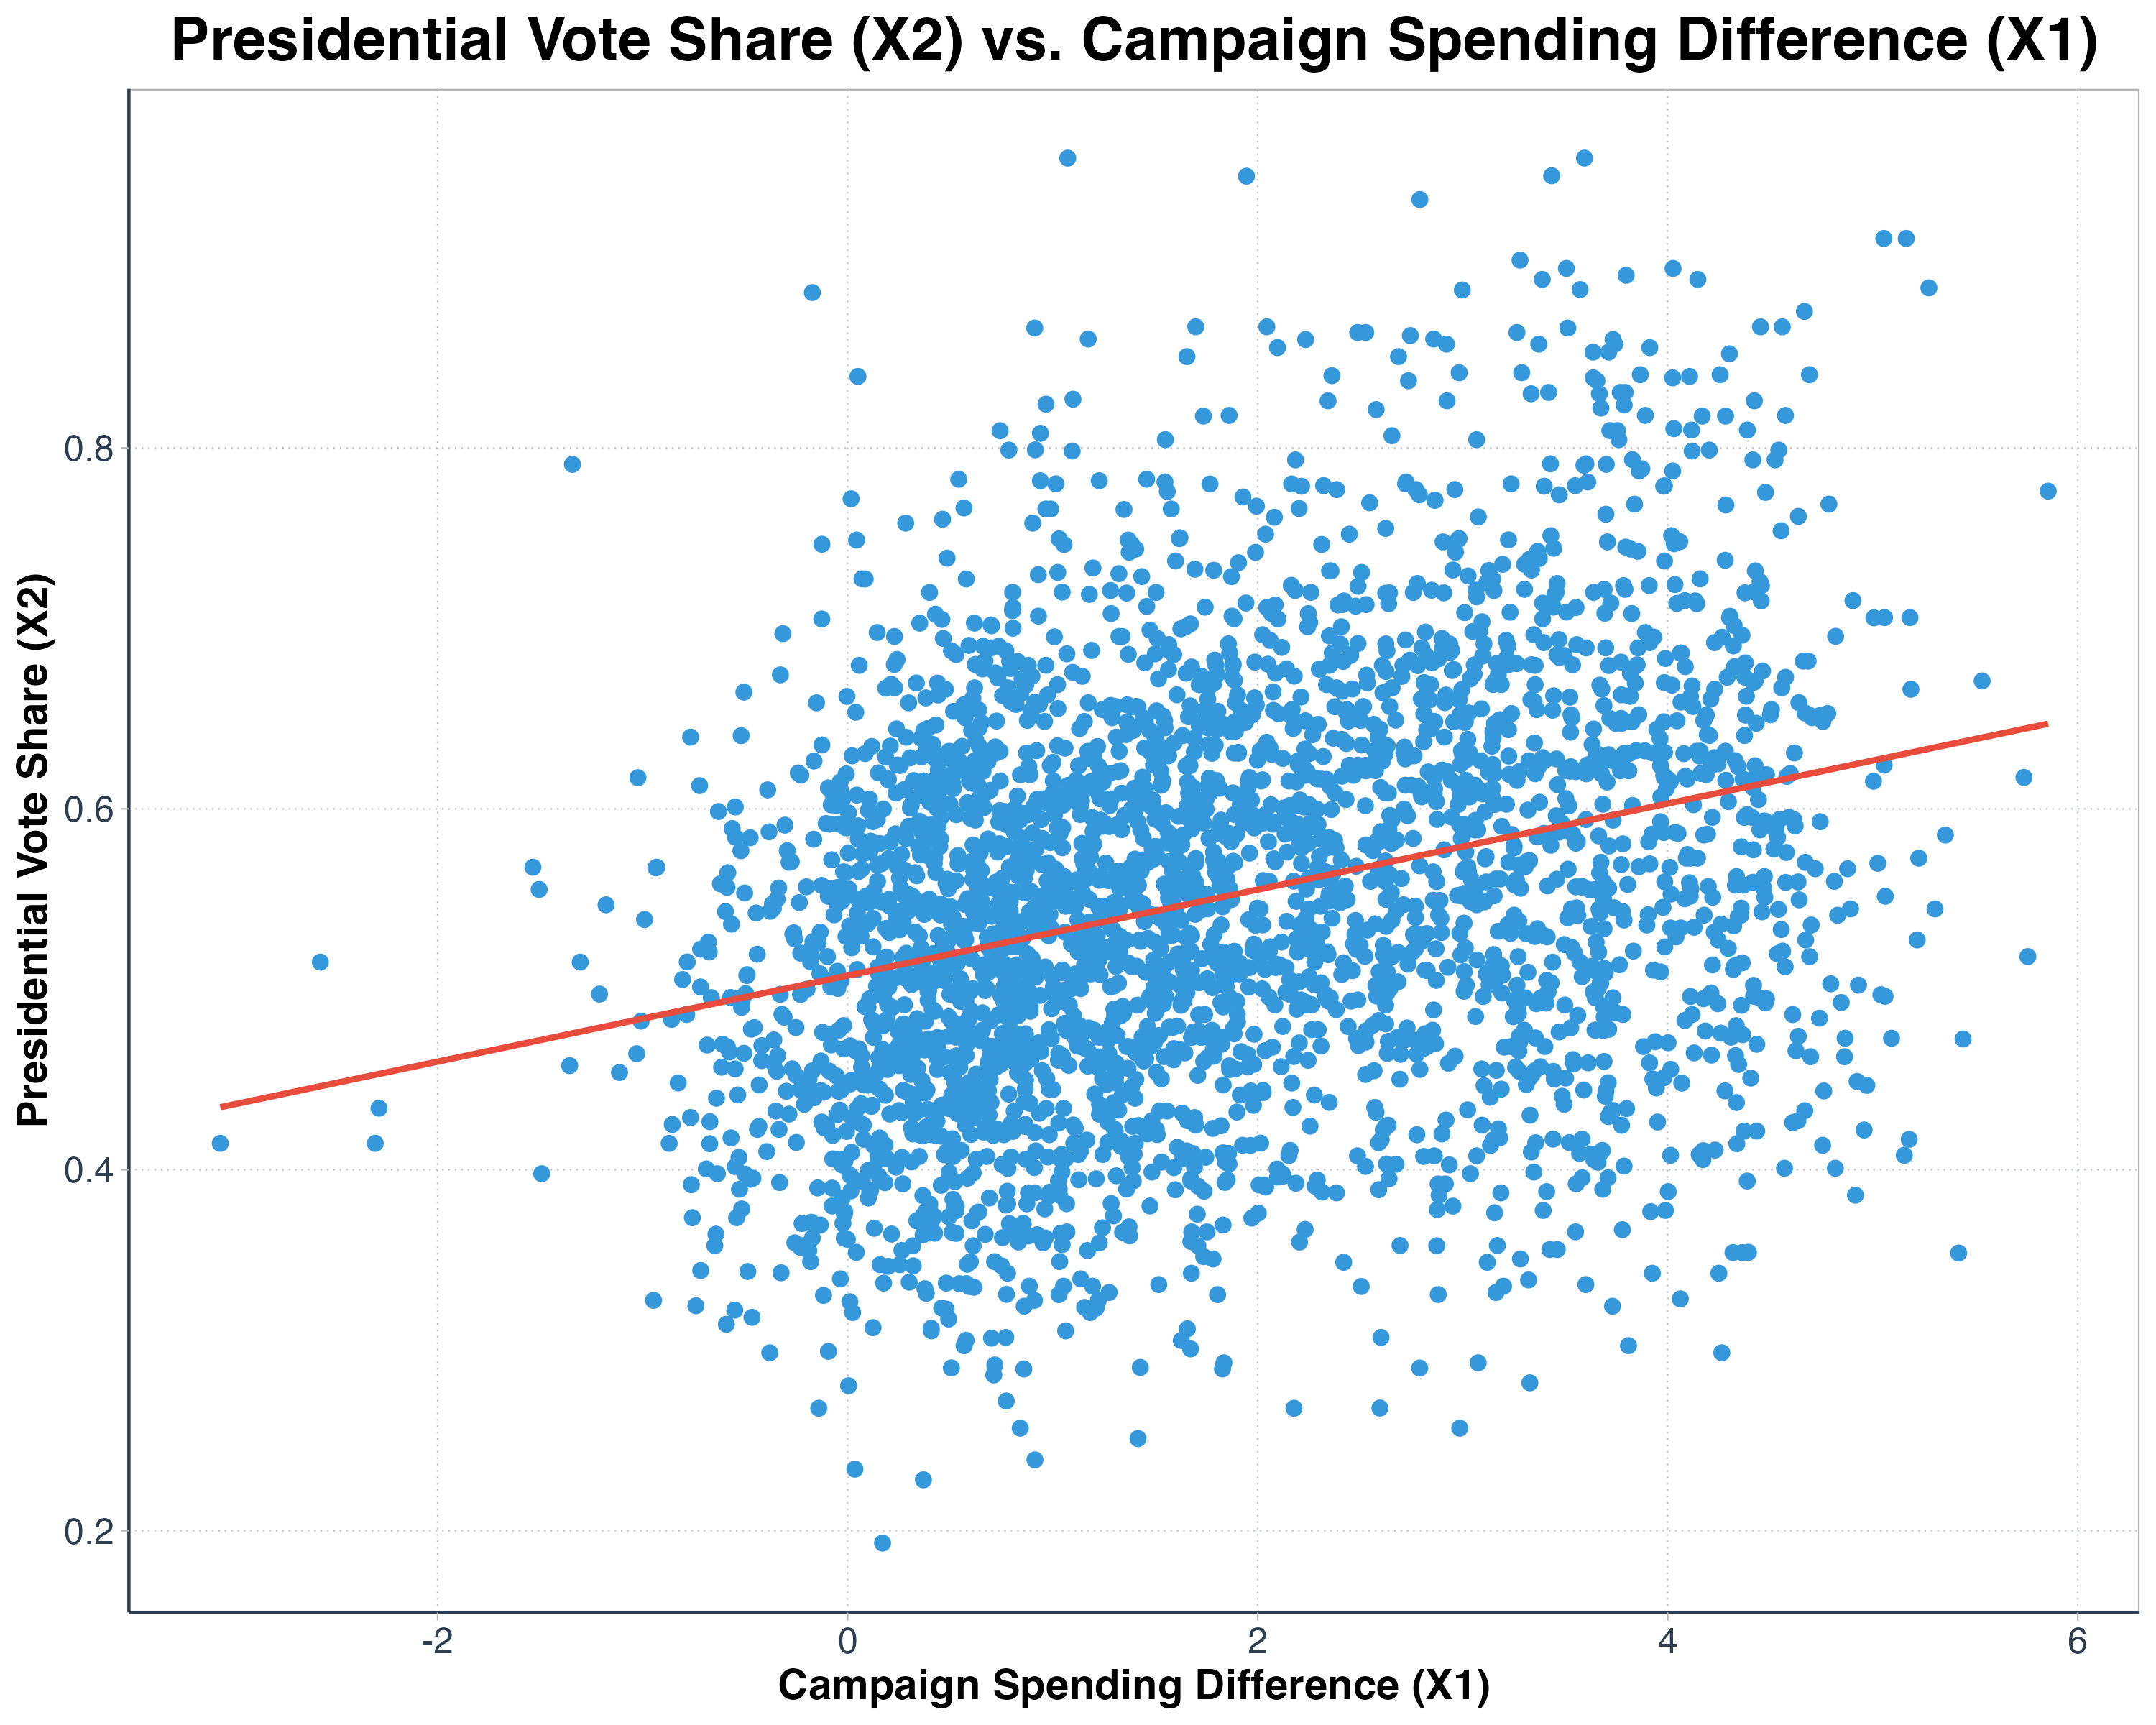
\includegraphics[width=.75\textwidth]{scatterplot_X2_X1_regression_line.png}
    \caption{\footnotesize X1 and X1.}
    \label{fig:plot_2}
    \smallskip
    \raggedright
    \textbf{Scatterplot Interpretation:}

    The scatterplot illustrates the spread of `X1` against `X2` with a fitted regression line. The line represents the linear relationship modeled by the regression analysis. The spread of points suggests there is variability that is not captured by `X1` alone, which is consistent with the R-squared value indicating a modest fit.
\end{figure}  

\newpage
\subsection{Save the residuals of the model in a separate object.}

Do it in R :
\begin{lstlisting}
# Save the residuals of the model in a separate object
residuals_X2_X1 <- resid(model_X2_X1)
# To view the first six residuals
head(residuals_X2_X1)
# To get a summary of the residuals
summary(residuals_X2_X1)
\end{lstlisting}
\newpage
\textbf{To represent R output in tabular form using LaTeX:}

\begin{table}[h!]
\centering
\begin{minipage}{.5\textwidth}
\centering
\begin{tabular}{|c|r|}
\hline
Observation & Residual \\
\hline
1 & 0.005605594 \\
2 & 0.037578519 \\
3 & -0.053134788 \\
4 & -0.052993694 \\
5 & -0.045842994 \\
6 & 0.074339701 \\
\hline
\end{tabular}
\caption{First six residuals of residuals\_X2\_X1.}
\label{tab:first_six_residuals}
\end{minipage}%
\begin{minipage}{.5\textwidth}
\centering
\begin{tabular}{|l|r|}
\hline
Statistic & Value \\
\hline
Minimum & -0.321965 \\
1st Quartile & -0.074069 \\
Median & -0.001018 \\
Mean & 0.000000 \\
3rd Quartile & 0.071507 \\
Maximum & 0.427435 \\
\hline
\end{tabular}
\caption{Summary statistics of residuals\_X2\_X1.}
\label{tab:summary_residuals}
\end{minipage}
\end{table}
\textbf{Residuals Analysis:}

The residuals' range from -0.32196 to 0.42743, with the median very close to zero, which is a good sign of a well-fitted model. The 1st and 3rd quartiles show that the middle 50\% of residuals are between -0.07407 and 0.07151, indicating that half of the residuals are within this range. The \texttt{head(residuals\_X2\_X1)} command shows the first six residuals from the model. This gives us a glimpse into the specific errors the model is making for individual predictions. The \texttt{summary(residuals\_X2\_X1)} provides a statistical summary of the residuals, confirming that the mean of the residuals is zero, which is an expected property of linear regression models.

\subsection{ Write the prediction equation.}

From the model summary, we can extract the intercept and slope coefficients to create the prediction equation. Additionally, we have the option to utilize R for this purpose.
 
Let's do it in R:
\begin{lstlisting}
# Write the prediction equation based on the model's coefficients
intercept_X2_X1 <- coef(model_X2_X1)[1]
slope_X2_X1 <- coef(model_X2_X1)[2]
prediction_equation_X2_X1 <- paste("X2 =", format(intercept_X2_X1, digits = 4), "+", format(slope_X2_X1, digits = 4), "* X1")
# Print out the prediction equation
print(prediction_equation_X2_X1)
\end{lstlisting}
\textbf{Now we have the prediction equation:}

\begin{equation}
X2 = 0.5076 + 0.02384 \times X1
\end{equation}
\textbf{The explanation of the prediction equation:}

The prediction equation indicates that the vote share of the presidential candidate (X2) also increases with the logged difference in campaign spending. For each one-unit increase in X1, X2 increases by 0.02384. The intercept (0.5076) represents the estimated presidential vote share when there is no difference in spending.
\section{Question 3}
\subsection{Run a regression where the outcome variable is voteshare and the explanatory variable is presvote.}
\textbf{Step 1: Rename 'voteshare' to 'Y' and 'presvote' to 'X2'. }
 Do it in R:
\begin{lstlisting}
# Step 1:Assuming 'voteshare' is already named 'Y' and 'presvote' is named 'X2' from previous steps.
# If not, rename them as follows:
names(inc.sub)[names(inc.sub) == "voteshare"] <- "Y"
names(inc.sub)[names(inc.sub) == "presvote"] <- "X2"

\end{lstlisting}
\textbf{Step 2:Run the Linear Regression:Fit a linear model with 'Y' as the dependent variable and 'X2' as the independent variable using the lm() function.}

Do it in R
\begin{lstlisting}
# Step 2: Run the regression with 'Y' as the outcome variable and 'X2' as the explanatory variable
# This models the relationship between the incumbent's vote share and the presidential vote share.
model_Y_X2 <- lm(Y ~ X2, data=inc.sub)

\end{lstlisting}
\textbf{Step 3:Output a summary of the linear regression model to get detailed statistics.}

Do it in R:
\begin{lstlisting}
# Step 3: Summarize the model to obtain the regression coefficients and other statistics.
# This summary provides details on the significance and strength of the relationship.
summary_Y_X2 <- summary(model_Y_X2)
print(summary_Y_X2) 
\end{lstlisting}
\textbf{Generate and display a summary of the linear regression model using R:}

\begin{center}
\begin{BVerbatim}
Call:
lm(formula = Y ~ X2, data = inc.sub)

Residuals:
     Min       1Q   Median       3Q      Max 
-0.27330 -0.05888  0.00394  0.06148  0.41365 

Coefficients:
            Estimate Std. Error t value Pr(>|t|)    
(Intercept) 0.441330   0.007599   58.08   <2e-16 ***
X2          0.388018   0.013493   28.76   <2e-16 ***
---
Signif. codes:  0 ‘***’ 0.001 ‘**’ 0.01 ‘*’ 0.05 ‘.’ 0.1 ‘ ’ 1

Residual standard error: 0.08815 on 3191 degrees of freedom
Multiple R-squared:  0.2058,	Adjusted R-squared:  0.2056 
F-statistic:   827 on 1 and 3191 DF,  p-value: < 2.2e-16
\end{BVerbatim}
\end{center}


\textbf{Use the R output to provide an explanation:}

A \textbf{linear regression model} was fitted with `Y` (incumbent's vote share) as the dependent variable and `X2` (presidential vote share) as the independent variable.

\textbf{Coefficients:} The model's intercept is approximately 0.4413, and the slope for `X2` is 0.388. These coefficients are statistically significant as indicated by the very low p-values.

\textbf{Model Fit:}The residual standard error is 0.08815, and the R-squared value is 0.2058. This means that approximately 20.58\% of the variance in the incumbent's vote share can be explained by the presidential vote share.
\subsection{Make a scatterplot of the two variables and add the regression line.}
Do it in R:
\begin{lstlisting}
# Create a scatterplot with 'X2' on the x-axis and 'Y' on the y-axis.
# The scatterplot will also include the regression line to visualize the relationship.
scatterplot_Y_X2 <- ggplot(inc.sub, aes(x=X2, y=Y)) +
  geom_point(color = "#3498db", shape = 19, size = 2) + # Blue points
  geom_smooth(method = "lm", color = "#e74c3c", se = FALSE, linetype = "solid", size = 1) + # Red regression line
  labs(title = "Incumbent's Vote Share (Y) vs. Presidential Vote Share (X2)",
       x = "Presidential Vote Share (X2)",
       y = "Incumbent's Vote Share (Y)") +
  theme_light() +
  theme(
    plot.title = element_text(hjust = 0.5, size = 20, face = "bold"),
    axis.title.x = element_text(size = 14, face = "bold"),
    axis.title.y = element_text(size = 14, face = "bold"),
    axis.text = element_text(size = 12, color = "#2c3e50"),
    axis.line = element_line(color = "#2c3e50"),
    panel.grid.major = element_line(color = "#bdc3c7", linetype = "dotted"),
    panel.grid.minor = element_blank(),
    legend.position = "none"
  )

# Save the scatterplot as a PNG file.
ggsave("scatterplot_Y_X2_regression_line.png", plot = scatterplot_Y_X2, width = 10, height = 8, dpi = 300)
\end{lstlisting}
\textbf{Now we have the scatterplot of the two variables and add the regression line:}
\begin{figure}[h!]
    \centering
    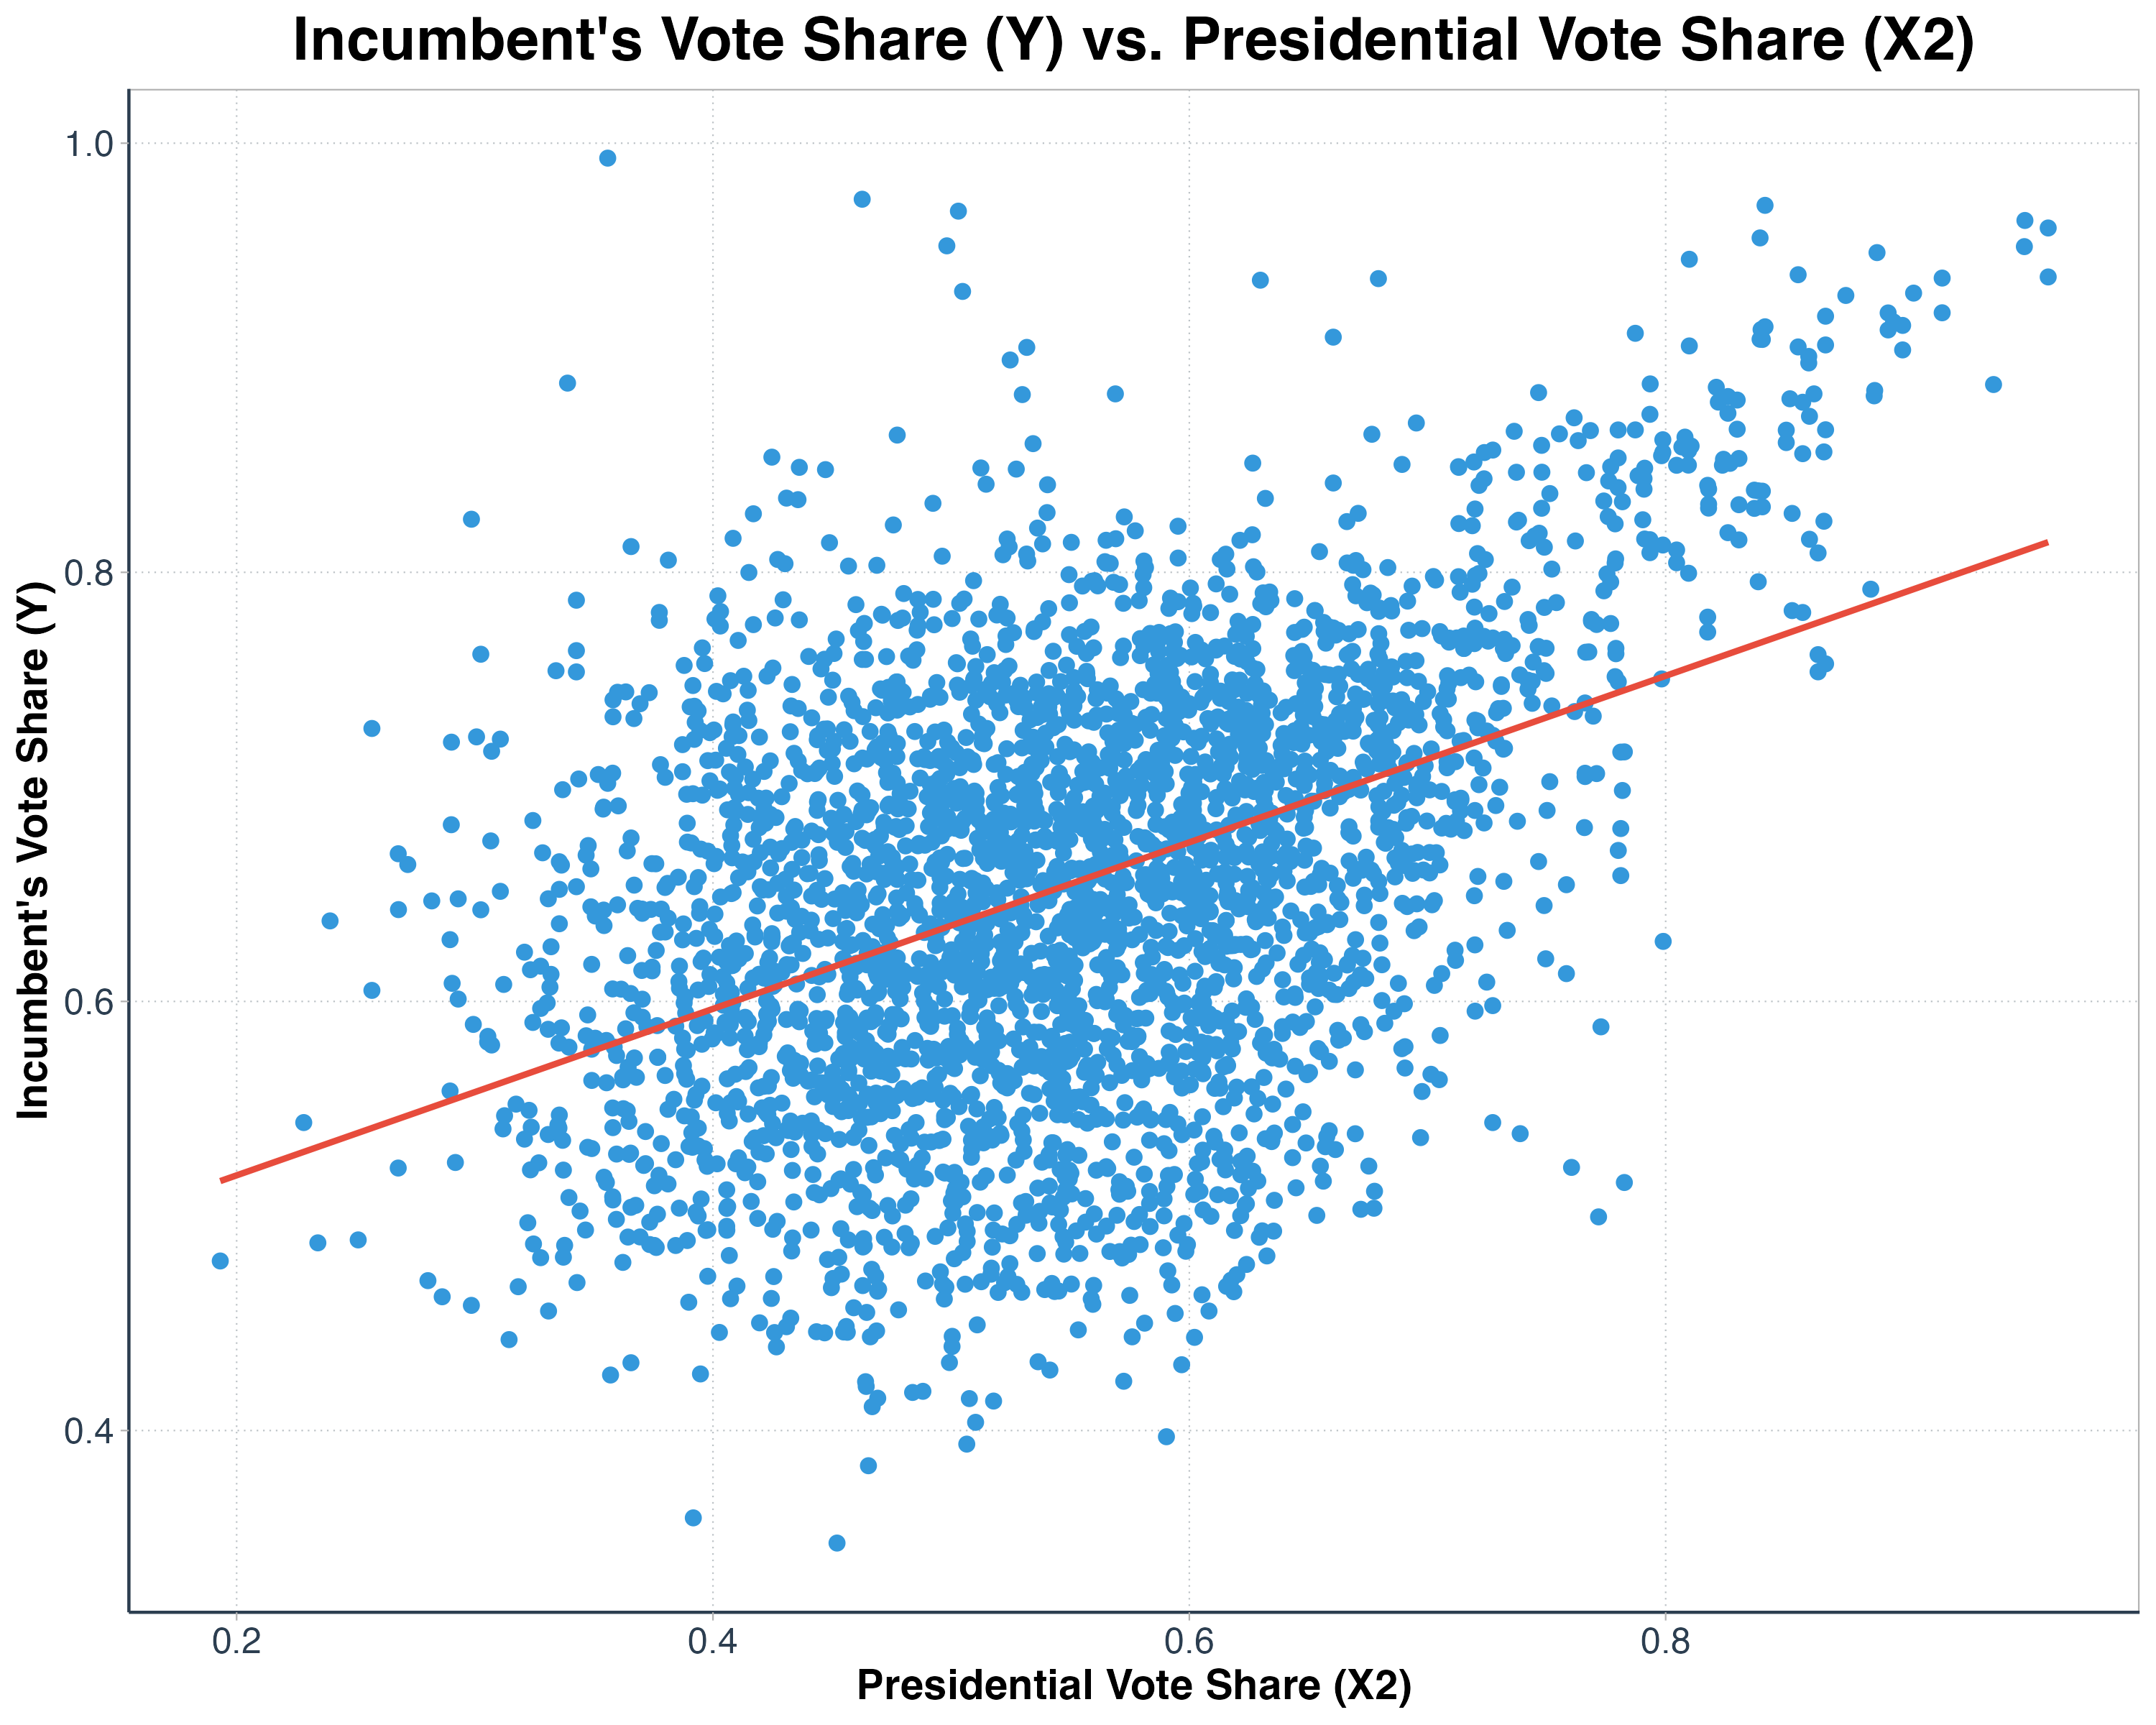
\includegraphics[width=.75\textwidth]{scatterplot_Y_X2_regression_line.png}
    \caption{\footnotesize Y and X2.}
    \label{fig:plot_3}
    \smallskip
    \raggedright
    \textbf{Scatterplot Interpretation:}
    
    The scatterplot visualizes the data points for `Y` and `X2`, with a regression line that shows the trend of the relationship. The positive slope indicates that as the presidential vote share increases, the incumbent's vote share also tends to increase.
\end{figure} 
\newpage
\subsection{Write the prediction equation.}
From the model summary, we can extract the intercept and slope coefficients to create the prediction equation. Additionally, we have the option to utilize R for this purpose.
 
Let's do it in R:
\begin{lstlisting}
#  Write the prediction equation based on the model's coefficients.
intercept_Y_X2 <- coef(model_Y_X2)[1]
slope_Y_X2 <- coef(model_Y_X2)[2]
prediction_equation_Y_X2 <- paste("Y =", format(intercept_Y_X2, digits = 4), "+", format(slope_Y_X2, digits = 4), "* X2")
print(prediction_equation_Y_X2)
\end{lstlisting}
\textbf{Now we have the prediction equation:}

\begin{equation}
Y = 0.4413 + 0.388 \times X2
\end{equation}

\textbf{The explanation of the prediction equation:}

This prediction equation indicates an observed relationship between the incumbent's vote share (Y) and the presidential vote share (X2). In this model, the incumbent's vote share is associated with the president's popularity, as represented by the vote share of the presidential candidate. The coefficient of 0.388 for X2 suggests that there is an association where an increase in the presidential vote share tends to be related to an increase in the incumbent's vote share.


\section{Question 4}
\subsection{Run a regression where the outcome variable is the residuals from Question 1 and the
explanatory variable is the residuals from Question 2.}
\textbf{Step 1: Use the residuals from Question 1 and 2}

Do it in R: 
\begin{lstlisting}
# Use the residuals from Question 1
residuals_Q1 <- resid(model)
# Use the residuals from Question 2
residuals_Q2 <- resid(model_X2_X1)
\end{lstlisting}
\textbf{Step 2:Run the regression with residuals from Question 1 as the outcome variable and residuals from Question 2 as the explanatory variable.}

Do it in R:
\begin{lstlisting}
# Run the regression with residuals from Question 1 as the outcome variable
# and residuals from Question 2 as the explanatory variable.
model_residuals <- lm(residuals_Q1 ~ residuals_Q2)
\end{lstlisting}
\textbf{Step 3:Output a summary of the linear regression model to get detailed statistics.}

Do it in R:
\begin{lstlisting}
#Summarize the model to obtain the regression coefficients and other statistics.
summary_residuals <- summary(model_residuals)
print(summary_residuals)
\end{lstlisting}
\textbf{Vote Share Residuals Correlation:}
Analyzing the relationship between the residuals from Questions 1 and 2 seeks to determine if there's a link between unexplained portions of the incumbent's and presidential candidate's vote shares. A significant relationship could imply shared influencing factors beyond campaign spending differences. Such insights are vital for uncovering hidden variables and enhancing models to better grasp the underlying dynamics of electoral outcomes.

\textbf{Generate and display a summary of the linear regression model using R:}
\begin{center}
\begin{BVerbatim}
Call:
lm(formula = residuals_Q1 ~ residuals_Q2)

Residuals:
     Min       1Q   Median       3Q      Max 
-0.25928 -0.04737 -0.00121  0.04618  0.33126 

Coefficients:
               Estimate Std. Error t value Pr(>|t|)    
(Intercept)  -5.934e-18  1.299e-03    0.00        1    
residuals_Q2  2.569e-01  1.176e-02   21.84   <2e-16 ***
---
Signif. codes:  0 ‘***’ 0.001 ‘**’ 0.01 ‘*’ 0.05 ‘.’ 0.1 ‘ ’ 1

Residual standard error: 0.07338 on 3191 degrees of freedom
Multiple R-squared:   0.13,	Adjusted R-squared:  0.1298 
F-statistic:   477 on 1 and 3191 DF,  p-value: < 2.2e-16   
\end{BVerbatim}
\end{center}


\textbf{Use the R output to provide an explanation:}

A \textbf{linear regression model} was fitted using the residuals from Question 1 (\texttt{residuals\_Q1}) as the dependent variable and the residuals from Question 2 (\texttt{residuals\_Q2}) as the independent variable.

\textbf{Coefficients:} The model's intercept is essentially zero ($-5.934 \times 10^{-18}$, which is numerically equivalent to 0 for all practical purposes), and the slope for \texttt{residuals\_Q2} is 0.2569. This suggests that there is a positive relationship between the residuals of the two models.

\textbf{Model Summary:} The residual standard error is 0.07338, indicating the standard deviation of the residuals from this new model. The R-squared value is 0.13, meaning that approximately 13\% of the variance in the residuals from the voteshare regression (Question 1) can be explained by the residuals from the presvote regression (Question 2).

\subsection{Make a scatterplot of the two residuals and add the regression line.}
Do it in R:
\begin{lstlisting}
# Create a scatterplot with residuals from Question 2 on the x-axis and residuals from Question 1 on the y-axis.
# The scatterplot will also include the regression line to visualize the relationship.
scatterplot_residuals <- ggplot(data.frame(residuals_Q1, residuals_Q2), aes(x=residuals_Q2, y=residuals_Q1)) +
  geom_point(color = "#3498db", shape = 19, size = 2) + # Blue points
  geom_smooth(method = "lm", color = "#e74c3c", se = FALSE, linetype = "solid", size = 1) + # Red regression line
  labs(title = "Residuals of Y vs. Residuals of X2",
       x = "Residuals of Presidential Vote Share (X2)",
       y = "Residuals of Incumbent's Vote Share (Y)") +
  theme_light() +
  theme(
    plot.title = element_text(hjust = 0.5, size = 20, face = "bold"),
    axis.title.x = element_text(size = 14, face = "bold"),
    axis.title.y = element_text(size = 14, face = "bold"),
    axis.text = element_text(size = 12, color = "#2c3e50"),
    axis.line = element_line(color = "#2c3e50"),
    panel.grid.major = element_line(color = "#bdc3c7", linetype = "dotted"),
    panel.grid.minor = element_blank(),
    legend.position = "none"
  )

# Save the scatterplot as a PNG file.
ggsave("scatterplot_residuals_regression_line.png", plot = scatterplot_residuals, width = 10, height = 8, dpi = 300)
\end{lstlisting}
\textbf{Now we have the scatterplot of the two residuals and add the regression line:}
\begin{figure}[h!]
    \centering
    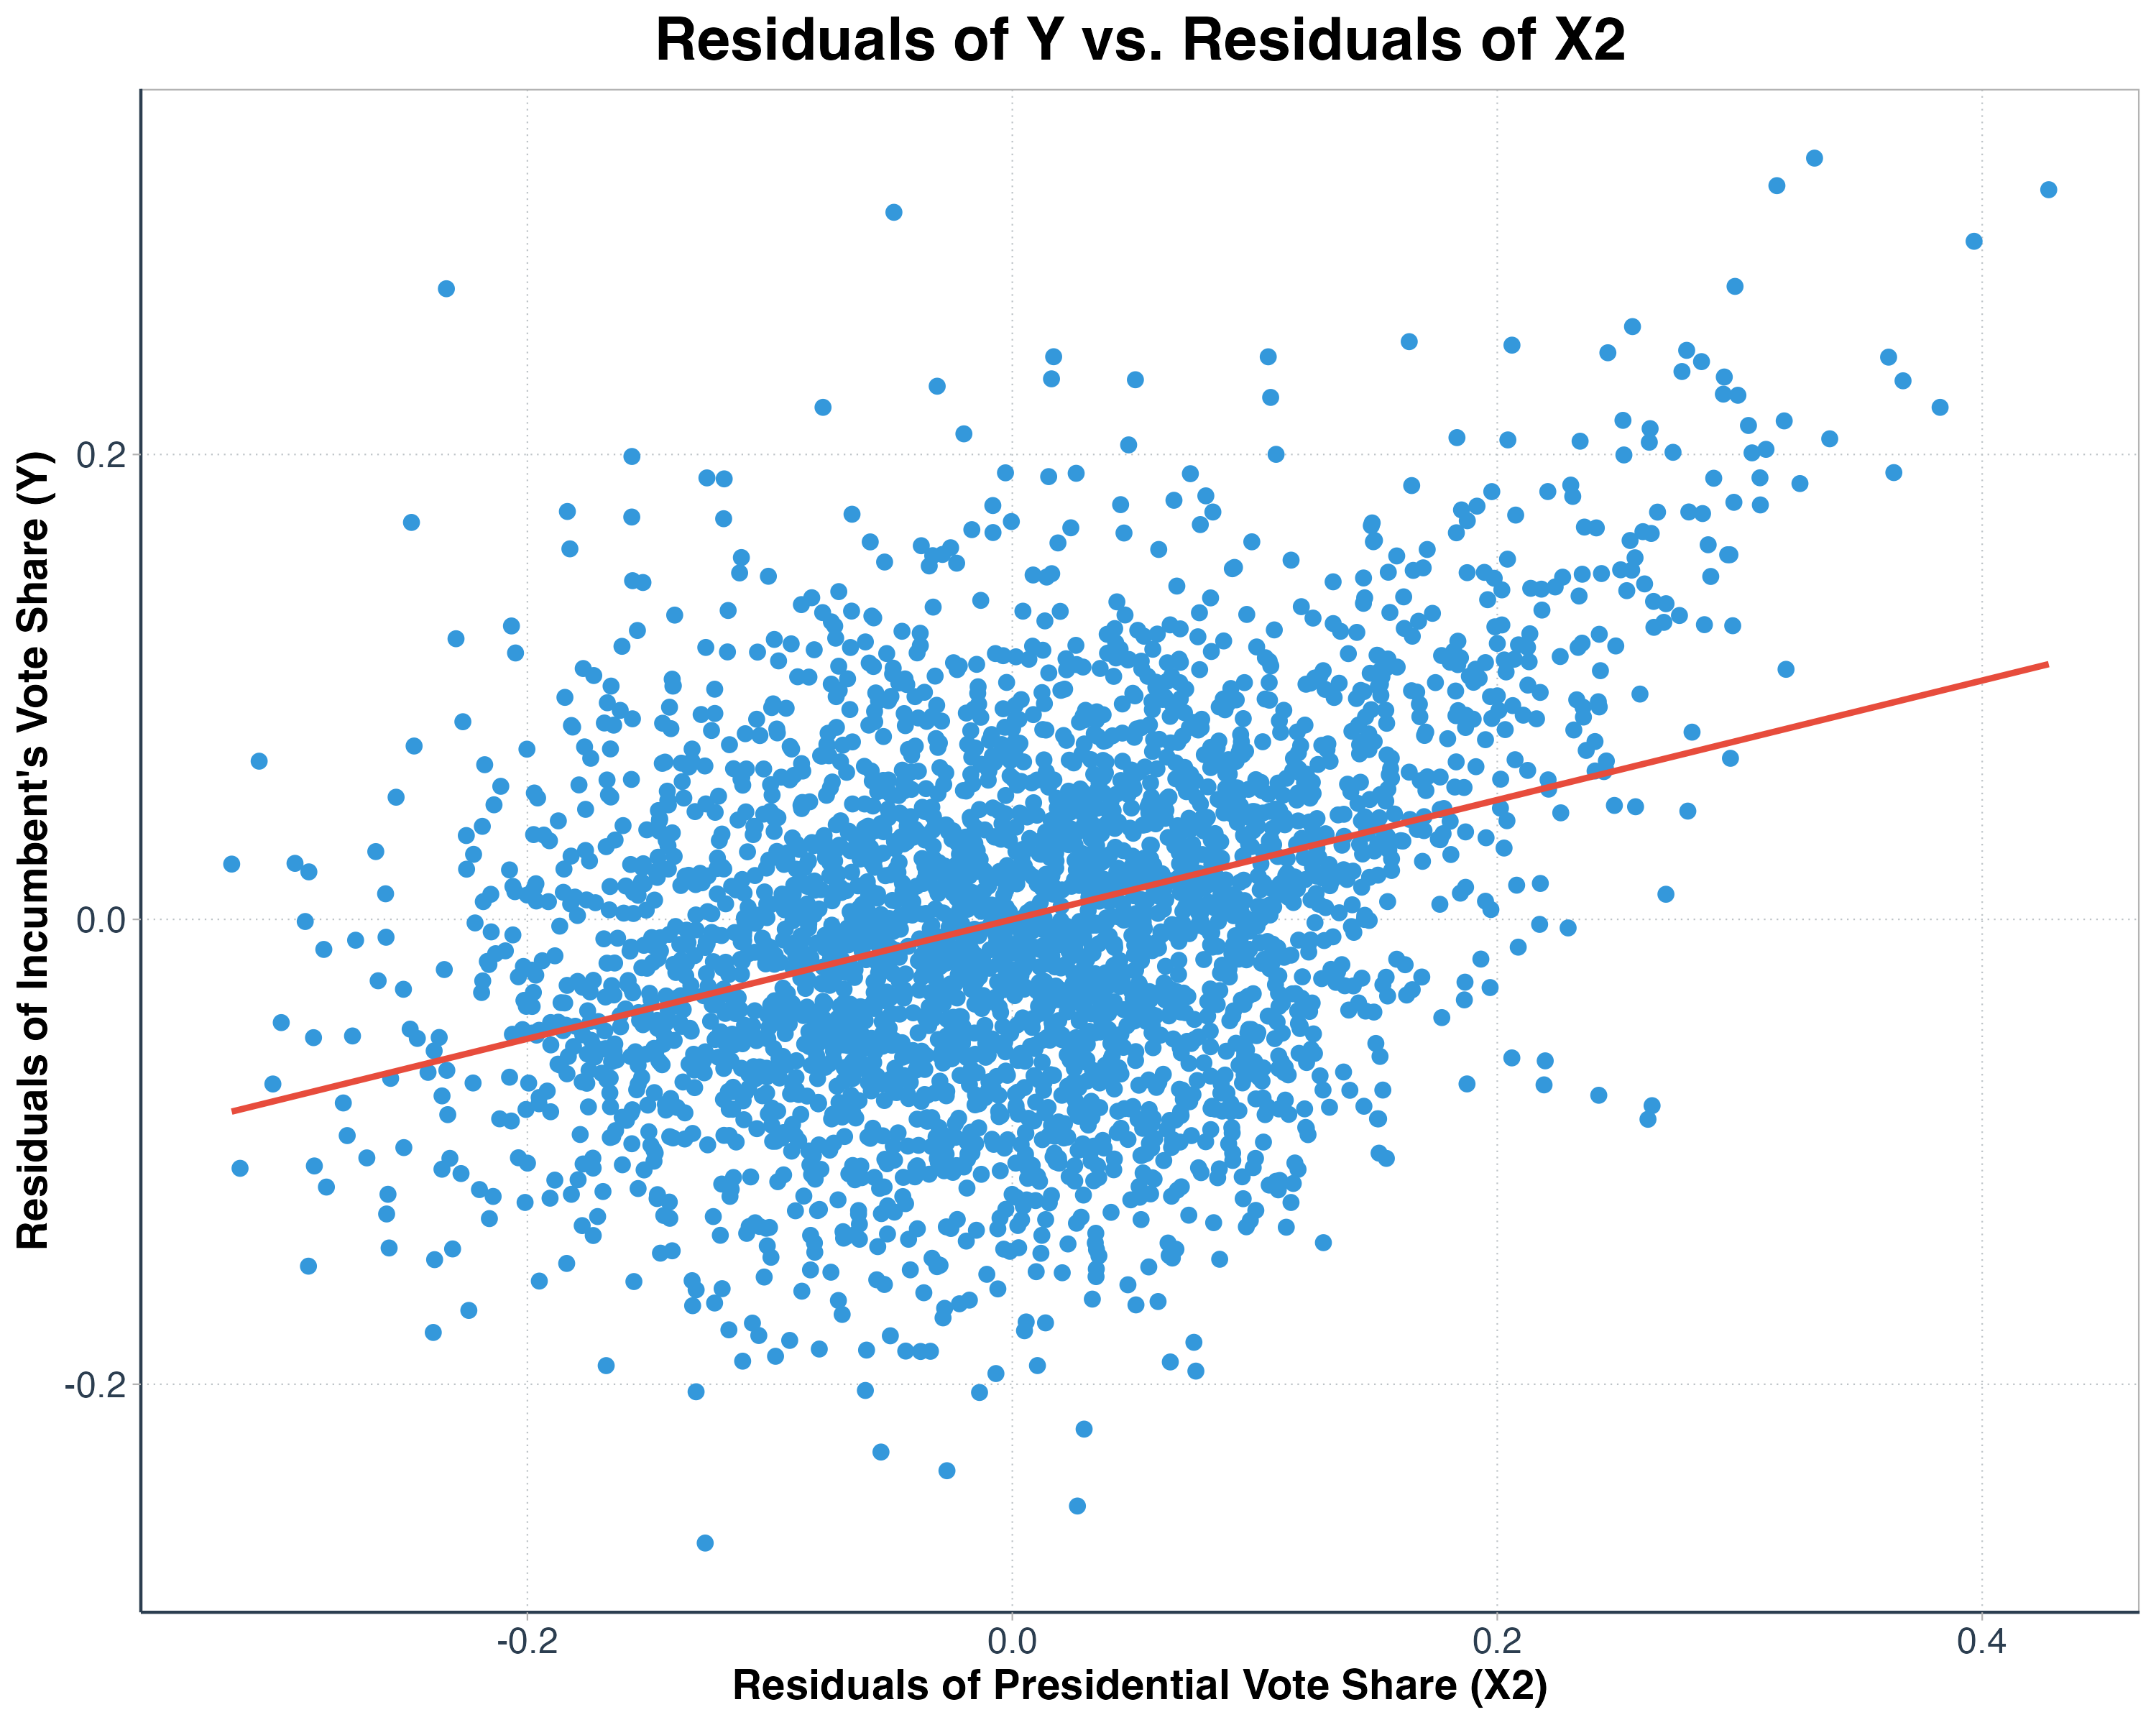
\includegraphics[width=.75\textwidth]{scatterplot_residuals_regression_line.png}
    \caption{\footnotesize Residuals of Incumbent's Vote Share (Y) and Residuals of Presidential Vote Share (X2).}
    \label{fig:plot_4}
    \smallskip
    \raggedright
    \textbf{Scatterplot Interpretation:}

    The scatterplot displays the relationship between the residuals from Question 1 and Question 2. The positive slope of the regression line indicates that as the residuals from the presidential vote share increase, the residuals from the incumbent's vote share also tend to increase.
\end{figure} 
\subsection{Write the prediction equation.}

From the model summary, we can extract the intercept and slope coefficients to create the prediction equation. Additionally, we have the option to utilize R for this purpose.

Let's do it in R:
\begin{lstlisting}
#Write the prediction equation based on the model's coefficients.
intercept_residuals <- coef(model_residuals)[1]
slope_residuals <- coef(model_residuals)[2]
prediction_equation_residuals <- paste("Residuals_Y =", format(intercept_residuals, digits = 4), "+", format(slope_residuals, digits = 4), "* Residuals_X2")
print(prediction_equation_residuals)
\end{lstlisting}
\textbf{Now we have the prediction equation is:}

\begin{equation}
\text{Residuals\_Y} = -5.934 \times 10^{-18} + 0.2569 \times \text{Residuals\_X2}
\end{equation}


 Since the intercept is statistically and practically insignificant, it can be simplified to:
  \begin{equation}
\text{Residuals\_Y} = 0.2569 \times \text{Residuals\_X2}
\end{equation}



This equation tells us that there is a positive association between the residuals of the two models. The presence of a significant relationship between these residuals indicates that the factors that cause variations in presidential vote share that are not explained by campaign spending differences also have a significant relationship with the variations in the incumbent’s vote share that are not explained by those same campaign spending differences. This could imply that there are underlying factors affecting both presidential vote share and incumbent vote share that are not captured by the campaign spending difference alone.
\newpage
\section{Question 5}
\subsection{Run a regression where the outcome variable is the incumbent's voteshare and the
explanatory variables are difflog and presvote.}
\textbf{Step 1:Run the Linear Regression:Fit a linear model with 'Y' as the dependent variable and both 'X1' and 'X2' as  independent variables using the lm() function.}

Do it in R:

\begin{lstlisting}
#Run the regression with Y as the outcome variable and both X1 and X2 as explanatory variables
model_Y_X1_X2 <- lm(Y ~ X1 + X2, data=inc.sub)
\end{lstlisting}
This may represent the multiple linear relationship:
\begin{equation}
    Y = \beta_0 + \beta_1 X1 + \beta_2 X2
\end{equation}
Where:
\begin{itemize}
    \item $Y$ represents the voteshare, the dependent variable in the model.
    \item $\beta_0$ is the intercept, representing the estimated voteshare when both difflog and presvote are zero. It serves as a baseline in the model.
    \item $\beta_1$ is the slope coefficient for $X1$, representing the effect of difflog (the logged difference in campaign spending) on voteshare. It indicates how a unit change in difflog affects voteshare, holding presvote constant.
    \item $X1$ (difflog) represents the logged difference in campaign spending.
    \item $\beta_2$ is the slope coefficient for $X2$, representing the effect of presvote (the president's vote share) on voteshare. It indicates how a unit change in presvote affects voteshare, holding difflog constant.
    \item $X2$ (presvote) represents the president's vote share.
\end{itemize}
\textbf{Step 2: Output a summary of the multiple linear regression to get detailed statistics.}

Do it in R:
\begin{lstlisting}
#Summarize the model to obtain the regression coefficients and other statistics.
summary_Y_X1_X2 <- summary(model_Y_X1_X2)
print(summary_Y_X1_X2)
\end{lstlisting}
\textbf{Generate and display a summary of the linear regression model using R:}

\begin{center}
\begin{BVerbatim}

Call:
lm(formula = Y ~ X1 + X2, data = inc.sub)

Residuals:
     Min       1Q   Median       3Q      Max 
-0.25928 -0.04737 -0.00121  0.04618  0.33126 

Coefficients:
             Estimate Std. Error t value Pr(>|t|)    
(Intercept) 0.4486442  0.0063297   70.88   <2e-16 ***
X1          0.0355431  0.0009455   37.59   <2e-16 ***
X2          0.2568770  0.0117637   21.84   <2e-16 ***
---
Signif. codes:  0 ‘***’ 0.001 ‘**’ 0.01 ‘*’ 0.05 ‘.’ 0.1 ‘ ’ 1

Residual standard error: 0.07339 on 3190 degrees of freedom
Multiple R-squared:  0.4496,	Adjusted R-squared:  0.4493 
F-statistic:  1303 on 2 and 3190 DF,  p-value: < 2.2e-16
\end{BVerbatim}
\end{center}
\nopagebreak
\textbf{Use the R output to provide an explanation:}

The model is a \textbf{multiple linear regression} with `voteshare` (Y) as the dependent variable, and `difflog` (X1) and `presvote` (X2) as independent variables. 

\textbf{Coefficients:}

\textbf{-Intercept (0.4486):} This is the estimated value of Y when both X1 and X2 are zero. Since a zero value for X1 and X2 is not meaningful within the context of this analysis (as it would imply no difference in spending and no votes for the president), the intercept here is more of a statistical artifact than a practical value.
   
\textbf{-X1 Coefficient (0.03554):}This value suggests that a one-unit increase in the logged difference in campaign spending (which is a multiplicative difference due to the logarithm) is associated with a 3.554 percentage point increase in the incumbent's vote share, holding the president's vote share constant.

 \textbf{  - X2 Coefficient (0.2569):}This implies that a one-unit increase in the president's vote share is associated with a 25.69 percentage point increase in the incumbent's vote share, holding the campaign spending difference constant. This is a substantial effect, indicating that the president's popularity may have a strong association with the incumbent's electoral success.

 \textbf{Residual Standard Error (RSE):} At 0.07339, the RSE is relatively low, which indicates that the model's predictions are, on average, within approximately 7.339 percentage points of the actual vote share values.
   
\textbf{R-squared (0.4496):} Approximately 44.96\% of the variation in the incumbent's vote share is explained by the model. This is a moderate amount of variance explained, which suggests that while these factors are important, there are other variables not included in the model that also affect the incumbent's vote share.
   
\textbf{F-statistic (1303):} The F-statistic is large, and the associated p-value is very small (< 2.2e-16), indicating that the model is statistically significant. This means that the independent variables collectively have a strong association with the dependent variable.

\textbf{Implications and Considerations}:The results suggest that both the campaign spending difference and the president's vote share have significant effects on the incumbent's vote share. It's important to consider that these variables may be correlated with each other; for instance, the president's popularity might influence campaign spending and vice versa.
 \subsection{Write the prediction equation.}
 From the model summary, we can extract the intercept and slope coefficients to create the prediction equation. Additionally, we have the option to utilize R for this purpose.
 
 Let's do it in R:
 \begin{lstlisting}
# Step 3: Write the prediction equation based on the model's coefficients
coefficients <- coef(model_Y_X1_X2)
prediction_equation_Y_X1_X2 <- paste("Y =", format(coefficients[1], digits = 4), "+",
format(coefficients[2], digits = 4), "* X1 +",
format(coefficients[3], digits = 4), "* X2")
print(prediction_equation_Y_X1_X2)
\end{lstlisting}
Now we have the prediction equation:

\begin{equation}
Y = 0.4486 + 0.03554 \times X1 + 0.2569 \times X2
\end{equation}

\textbf{The explanation of the prediction equation:}

This equation indicates that the incumbent's vote share (Y) is positively associated with both the logged difference in campaign spending (X1) and the president's vote share (X2).
\subsection{What is it in this output that is identical to the output in Question 4? Why do you
think this is the case?}

The identical element in the outputs of Questions 4 and 5 is the\textbf{ coefficient for `X2` (presvote)}, consistently at \textbf{0.2569.} This similarity highlights a fundamental aspect of regression analysis, specifically regarding the interpretation of coefficients in \textbf{multiple regression models}.

In Question 4, the regression involved the residuals of `Y` (after accounting for `X1`) against the residuals of `X2` (also after accounting for `X1`). This analysis essentially isolated the part of `Y` not explained by `X1`, examining how it relates to the portion of `X2` unexplained by `X1`. The focus was on the \textbf{unique contribution of `X2` to `Y`, independent of `X1`.}

Question 5’s multiple regression model, where both `X1` and `X2` are included, reveals a similar story but through a direct approach. \textbf{The coefficient for `X2` in this model quantifies its unique effect on `Y`, while controlling for `X1`. The presence of `X1` in the model does not alter the distinct impact of `X2` on `Y`, }which is why the coefficient of `X2` remains unchanged from the analysis in Question 4.

This consistency in the coefficient of `X2` across both analyses underlines the \textbf{robustness of the relationship }between the p\textbf{resident’s popularity and the incumbent’s electoral success.} It suggests that the influence of presidential popularity on the incumbent's vote share is a distinct and significant factor, irrespective of the differences in campaign spending. This insight is crucial as it implies that \textbf{factors influencing presidential popularity might also have direct repercussions on the electoral outcomes of incumbents, beyond what can be attributed to campaign spending alone.}

\end{document}

